\documentclass[a4paper, 11pt, oneside]{article}

\usepackage[utf8]{inputenc}
\usepackage[T1]{fontenc}
\usepackage[french]{babel}
\usepackage{array}
\usepackage{shortvrb}
\usepackage{listings}
\usepackage[fleqn]{amsmath}
\usepackage{amsfonts}
\usepackage{fullpage}
\usepackage{enumerate}
\usepackage{graphicx}             % import, scale, and rotate graphics
\usepackage{subfigure}            % group figures
\usepackage{alltt}
\usepackage{url}
\usepackage{indentfirst}
\usepackage{eurosym}
\usepackage{listings}
\usepackage{color}
\usepackage[table,xcdraw,dvipsnames]{xcolor}

% Change le nom par défaut des listing
\renewcommand{\lstlistingname}{Extrait de Code}

% Change la police des titres pour convenir à votre seul lecteur
\usepackage{sectsty}
\allsectionsfont{\sffamily\mdseries\upshape} 
% Idem pour la table des matière.
\usepackage[nottoc,notlof,notlot]{tocbibind} 
\usepackage[titles,subfigure]{tocloft} 
\renewcommand{\cftsecfont}{\rmfamily\mdseries\upshape}
\renewcommand{\cftsecpagefont}{\rmfamily\mdseries\upshape} 

\definecolor{mygray}{rgb}{0.5,0.5,0.5}
\newcommand{\coms}[1]{\textcolor{MidnightBlue}{#1}}

\lstset{
    language=C, % Utilisation du langage C
    commentstyle={\color{MidnightBlue}}, % Couleur des commentaires
    frame=single, % Entoure le code d'un joli cadre
    rulecolor=\color{black}, % Couleur de la ligne qui forme le cadre
    stringstyle=\color{RawSienna}, % Couleur des chaines de caractères
    numbers=left, % Ajoute une numérotation des lignes à gauche
    numbersep=5pt, % Distance entre les numérots de lignes et le code
    numberstyle=\tiny\color{mygray}, % Couleur des numéros de lignes
    basicstyle=\tt\footnotesize, 
    tabsize=3, % Largeur des tabulations par défaut
    keywordstyle=\tt\bf\footnotesize\color{Sepia}, % Style des mots-clés
    extendedchars=true, 
    captionpos=b, % sets the caption-position to bottom
    texcl=true, % Commentaires sur une ligne interprétés en Latex
    showstringspaces=false, % Ne montre pas les espace dans les chaines de caractères
    escapeinside={(>}{<)}, % Permet de mettre du latex entre des <( et )>.
    inputencoding=utf8,
    literate=
  {á}{{\'a}}1 {é}{{\'e}}1 {í}{{\'i}}1 {ó}{{\'o}}1 {ú}{{\'u}}1
  {Á}{{\'A}}1 {É}{{\'E}}1 {Í}{{\'I}}1 {Ó}{{\'O}}1 {Ú}{{\'U}}1
  {à}{{\`a}}1 {è}{{\`e}}1 {ì}{{\`i}}1 {ò}{{\`o}}1 {ù}{{\`u}}1
  {À}{{\`A}}1 {È}{{\`E}}1 {Ì}{{\`I}}1 {Ò}{{\`O}}1 {Ù}{{\`U}}1
  {ä}{{\"a}}1 {ë}{{\"e}}1 {ï}{{\"i}}1 {ö}{{\"o}}1 {ü}{{\"u}}1
  {Ä}{{\"A}}1 {Ë}{{\"E}}1 {Ï}{{\"I}}1 {Ö}{{\"O}}1 {Ü}{{\"U}}1
  {â}{{\^a}}1 {ê}{{\^e}}1 {î}{{\^i}}1 {ô}{{\^o}}1 {û}{{\^u}}1
  {Â}{{\^A}}1 {Ê}{{\^E}}1 {Î}{{\^I}}1 {Ô}{{\^O}}1 {Û}{{\^U}}1
  {œ}{{\oe}}1 {Œ}{{\OE}}1 {æ}{{\ae}}1 {Æ}{{\AE}}1 {ß}{{\ss}}1
  {ű}{{\H{u}}}1 {Ű}{{\H{U}}}1 {ő}{{\H{o}}}1 {Ő}{{\H{O}}}1
  {ç}{{\c c}}1 {Ç}{{\c C}}1 {ø}{{\o}}1 {å}{{\r a}}1 {Å}{{\r A}}1
  {€}{{\euro}}1 {£}{{\pounds}}1 {«}{{\guillemotleft}}1
  {»}{{\guillemotright}}1 {ñ}{{\~n}}1 {Ñ}{{\~N}}1 {¿}{{?`}}1
}
\newcommand{\tablemat}{~}

%%%%%%%%%%%%%%%%% TITRE %%%%%%%%%%%%%%%%
\newcommand{\GrNbr}{s180498-s170220}
\newcommand{\PrenomUN}{Martin}
\newcommand{\NomUN}{RANDAXHE}
\newcommand{\PrenomDEUX}{Cyril}
\newcommand{\NomDEUX}{RUSSE}
\renewcommand{\tablemat}{\tableofcontents}

\title{\textbf{MATH1222-3 - Introduction aux Processus Stochastiques}\\Projet Chaîne de Markov en temps discret}
\author{Groupe \GrNbr : \PrenomUN~\textsc{\NomUN}, \PrenomDEUX~\textsc{\NomDEUX}}
\date{}
\begin{document}
\maketitle
\newpage
\tablemat
\newpage

%%%%%%%%%%%%%%%%%%%%%%%%%%%%%%%%%%%%%%%%%%%%%%%%
\section{\textbf{Modèle(s) exact(s) à deux individus}}
\subsection{Question 1}

Etant donné que nous sommes dans un cas où nous avons deux individus 
pouvant chacun être soit Susceptible(S), Infectieux(I) ou Immunisés(R).

Il existe $3^2$ possibilités d'états des individus.
Ils se composent de 8 états transitoires 
\begin{enumerate}
    \item SI
    \item RS 
    \item II 
    \item IR 
    \item RI 
    \item IS 
    \item RR 
    \item SR 
    \\et 1 état persistant
    \item SS
\end{enumerate}
Voici ensuite le graphe de transition associé à la chaine de Markov.
\begin{figure}[h]
    \centering
    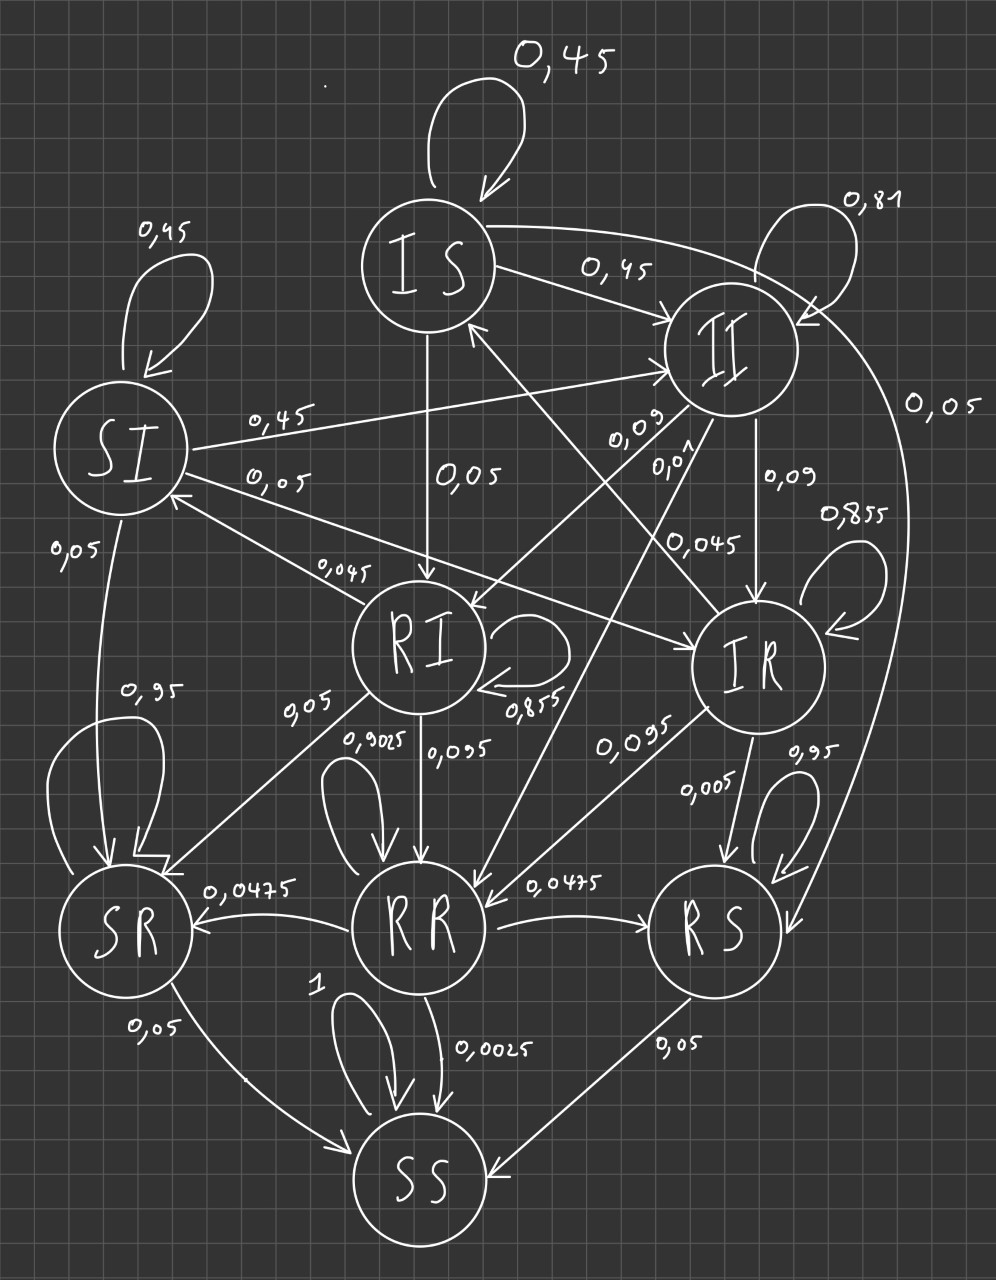
\includegraphics[scale=0.55]{graphe_question1.jpg}
    \caption{Graphe de transition associé à la chaine de Markov}
\end{figure}

\subsection{Question 2}

Nous allons maintenant caractériser la chaine. 
Elle se compose de 5 classes différentes :
$C1 = \{IS, II, SI, RI, IR\}
\\C2 = \{RS\}
\\C3 = \{SR\}
\\C4 = \{RR\}
\\C5 = \{SS\}$
\\Les classes C1, C2, C3 et C4 sont des classes de passages 
et la classe C5 est une classe finale.
Etant donné que nous avons ces 5 classes, la chaine n'est pas irréductible.
Elle n'est pas non plus périodique. Si elle n'est pas irréductible et pas périodique 
elle n'est pas régulière. Elle est par ailleurs absobante étant donné que la classe 
C5 est finale.

\subsection{Question 3}

Afin de trouver les proportions des différents états, il nous suffit de 
calculer pour chaque pas de temps les proportions de chaque état à l'aide de 
la puissance correspondante de la matrice de transition. Ce qui amène au graphique 
ci-dessous. On observe bien que l'on tend vers une disparition du virus et donc 
au fur et à mesure du temps on observe que S tend vers 1, en effet, si 
le virus disparait la totalité de la distribution tend à se retrouver dans S.
(Détail des opérations pour obtenir ce graphique dans le script )

\begin{figure}[h]
    \centering
    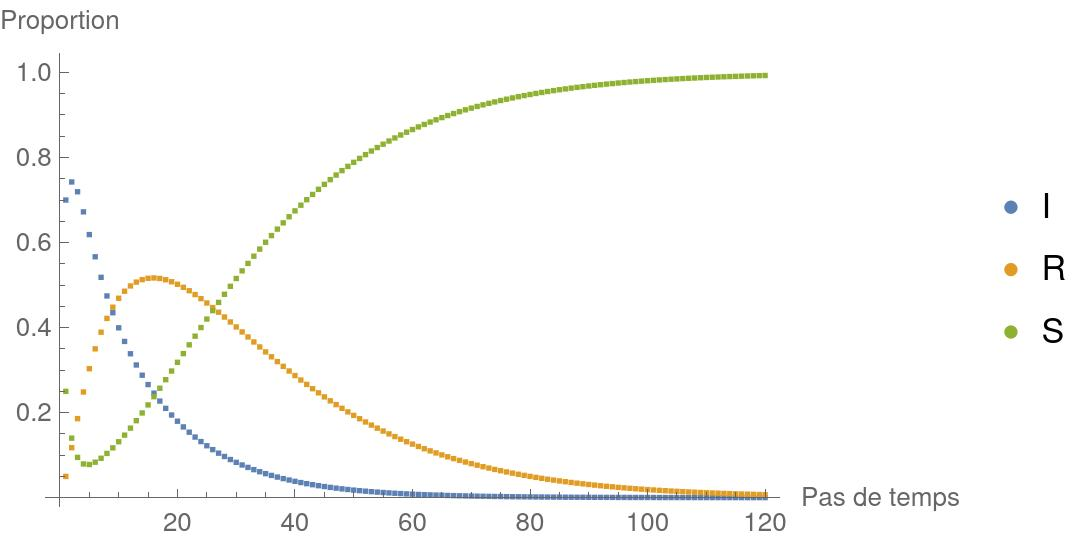
\includegraphics[scale=0.95]{graphiqueSIR.jpg}
    \caption{Proportion des différents états en fonction du temps}
\end{figure}

\subsection{Question 4}
\subsubsection{Calcul du temps de disparition du virus}
La Figure 3 représente la matrice de transition.

\begin{figure}[h]
    \centering
    \hspace{+0.5cm}{
    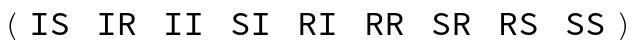
\includegraphics[scale=0.95]{vecteur_ligne.jpg}}\\
    
\includegraphics[scale=0.5]{ordre_matrice_transitionQ4.jpg}
    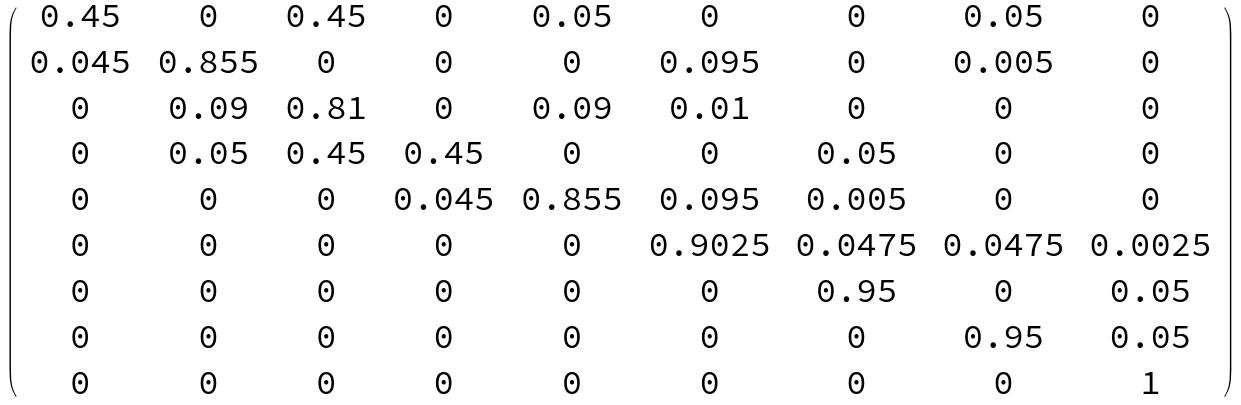
\includegraphics[scale=0.5]{matriceTansition_Q4.jpg}
    \caption{Matrice de transition}
\end{figure}
En utilisant le théorème des temps moyens d'atteinte, à partir de cette 
matrice de transition, nous avons trouvé qu'en moyenne avec comme situation initiale 
"SI", il faut en moyenne 10,543 pas de temps pour atteindre "RR" et 16,543 pas 
de temps pour atteindre "SR" ou "RS". Ce qui donne en moyenne 14,543 pas de temps pour atteindre 
un de ces 3 cas. Et celà correspond donc au temps moyen nécessaire à la disparition  totale du virus car 
à partir du moment où l'on atteint un de ces 3 états, il n'est plus possible d'avoir un nouveau cas 
infectieux.

\subsubsection{Analyse de l'impact des paramètres sur le temps de disparition du virus}
Afin d'atteindre un état de disparition du virus, il est interessant d'avoir une faible chance de passer d'un 
statut sain : Susceptible ou Immunisés. Et une forte de chance que les cas Infectieux guérissent. 
Dorénavant, en terme de paramètres, il est interessant d'avoir de très petites valeurs pour 
$\beta$ et $\alpha$. En revanche un grande valeur de $\mu$ serait préférable.

\subsection{Question 5}

\begin{itemize}
    \item a)
    \\    \begin{figure}[h]
        \centering
        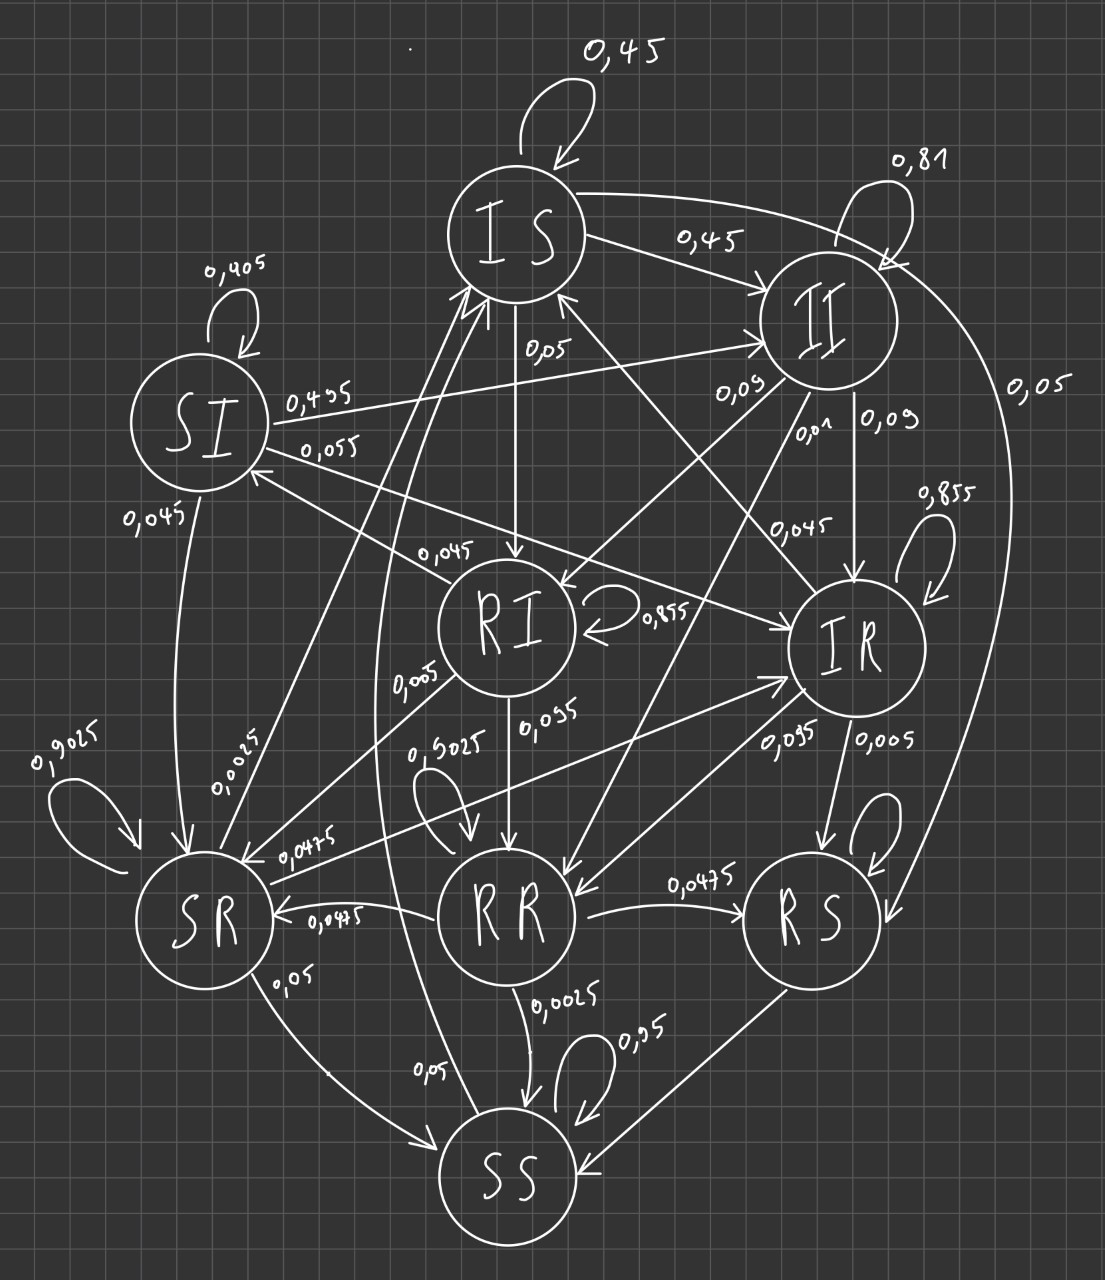
\includegraphics[scale=0.55]{graphe2Q5.jpg}
        \caption{Nouveau graphe de transition prenant $\delta$ en compte}
    \end{figure}
    \item b)
    \\Afin de calculer le pourcentage de temps passé par chaque individu 
    dans l'état infectieux, nous devons trouver, étant donné que la chaine de Markov 
    est régulière, le vecteur de distribution obtenu en calculant la limite pour n qui 
    tend vers l'infini de la matrice de transition à la puissance n.(Figure 4)
    \begin{figure}[h]
        \centering
        
\includegraphics[scale=0.55]{ordre_matrice_transitionQ4.jpg}
        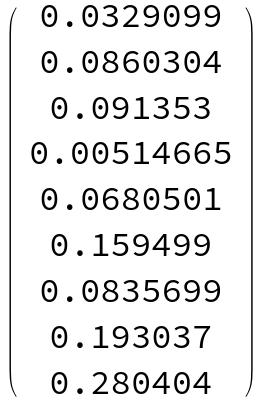
\includegraphics[scale=0.55]{vecteurQ5.jpg}
        \caption{Vecteur de distribution lors de l'état stationnaire de la chaine de Markov régulière}
    \end{figure}
    \\Pour la première personne, nous nous interesserons aux 3 premières lignes du 
    vecteur. Ainsi, celle-ci passera en moyenne 21,03\% de son temps dans l'état infectieux.
    Dans le cas du deuxième, nous avons besoin des lignes 3 à 5 et on obtient 16,45\% de temps 
    dans l'état infectieux. 
    \\Nous observons donc bien un plus grand pourcentage 
    pour la première personne ayant d'autres contact extérieur impliquant un 
    plus grande probabilité d'être infecté.

\end{itemize}









\end{document}
